\chapter{Management}

In this section, management of the platform will be discussed. In earlier versions of the platform, it can only be managed with people who has understanding of command line interface\footnote{https://en.wikipedia.org/wiki/Command-line_interface}. It was blocking feature, limiting usage and management of the platform. As the platform used in lectures by instructors and contents of the challenges are customized based on curricula of the courses. The management of the platform must be informative, user friendly and self explained. Hence, web interface has been developed, it brought great convenience and safety. 
The command line tool was providing the actions given in the Figure 4.1

\begin{figure}[htbp]
\centerline{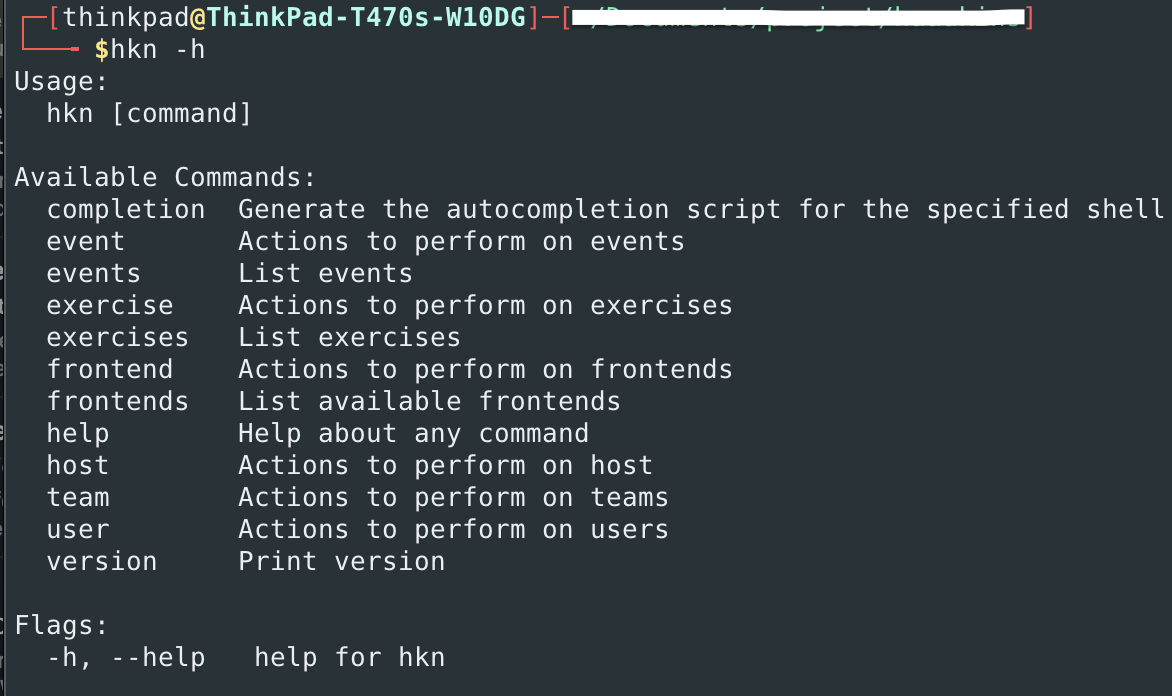
\includegraphics[scale=.6]{figures/cli.png}}
\caption{Command Line Tool Options of Haaukins }
\label{fig}
\end{figure}

The CLI can be fun to play when you know otherwise it might be headache. Simple event creation command with CLI is shown in Figure 4.2
\begin{figure}[htbp]
\centerline{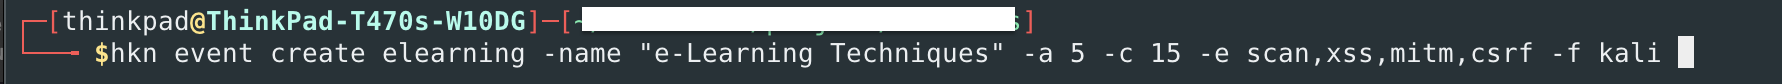
\includegraphics[scale=.6]{figures/create-event.png}}
\caption{Creation of an event through CLI }
\label{fig}
\end{figure}
\newpage
The problem should be observed from the Figure 4.2, the command does not explain itself, there are some challenges passed with "-e" flag. All the flags passed as argument to CLI tool needs to known by creator of an event. The command is creating an event with some group of challenges (scan, xss, mitm, csrf), with availability of five, capacity of 15, and name of the event is "e-Learning Techniques". However, all these information needs to known at first glance when start to manage the platform. Even more, all the challenge information should be given when creating an event. Otherwise, event creator might create an event blindly, randomly without a knowledge about what they want. 
In order to prevent such terrible situations, web based solution is introduced to the platform with all detailed information of challenges and fields. 

\begin{figure}[htbp]
\centerline{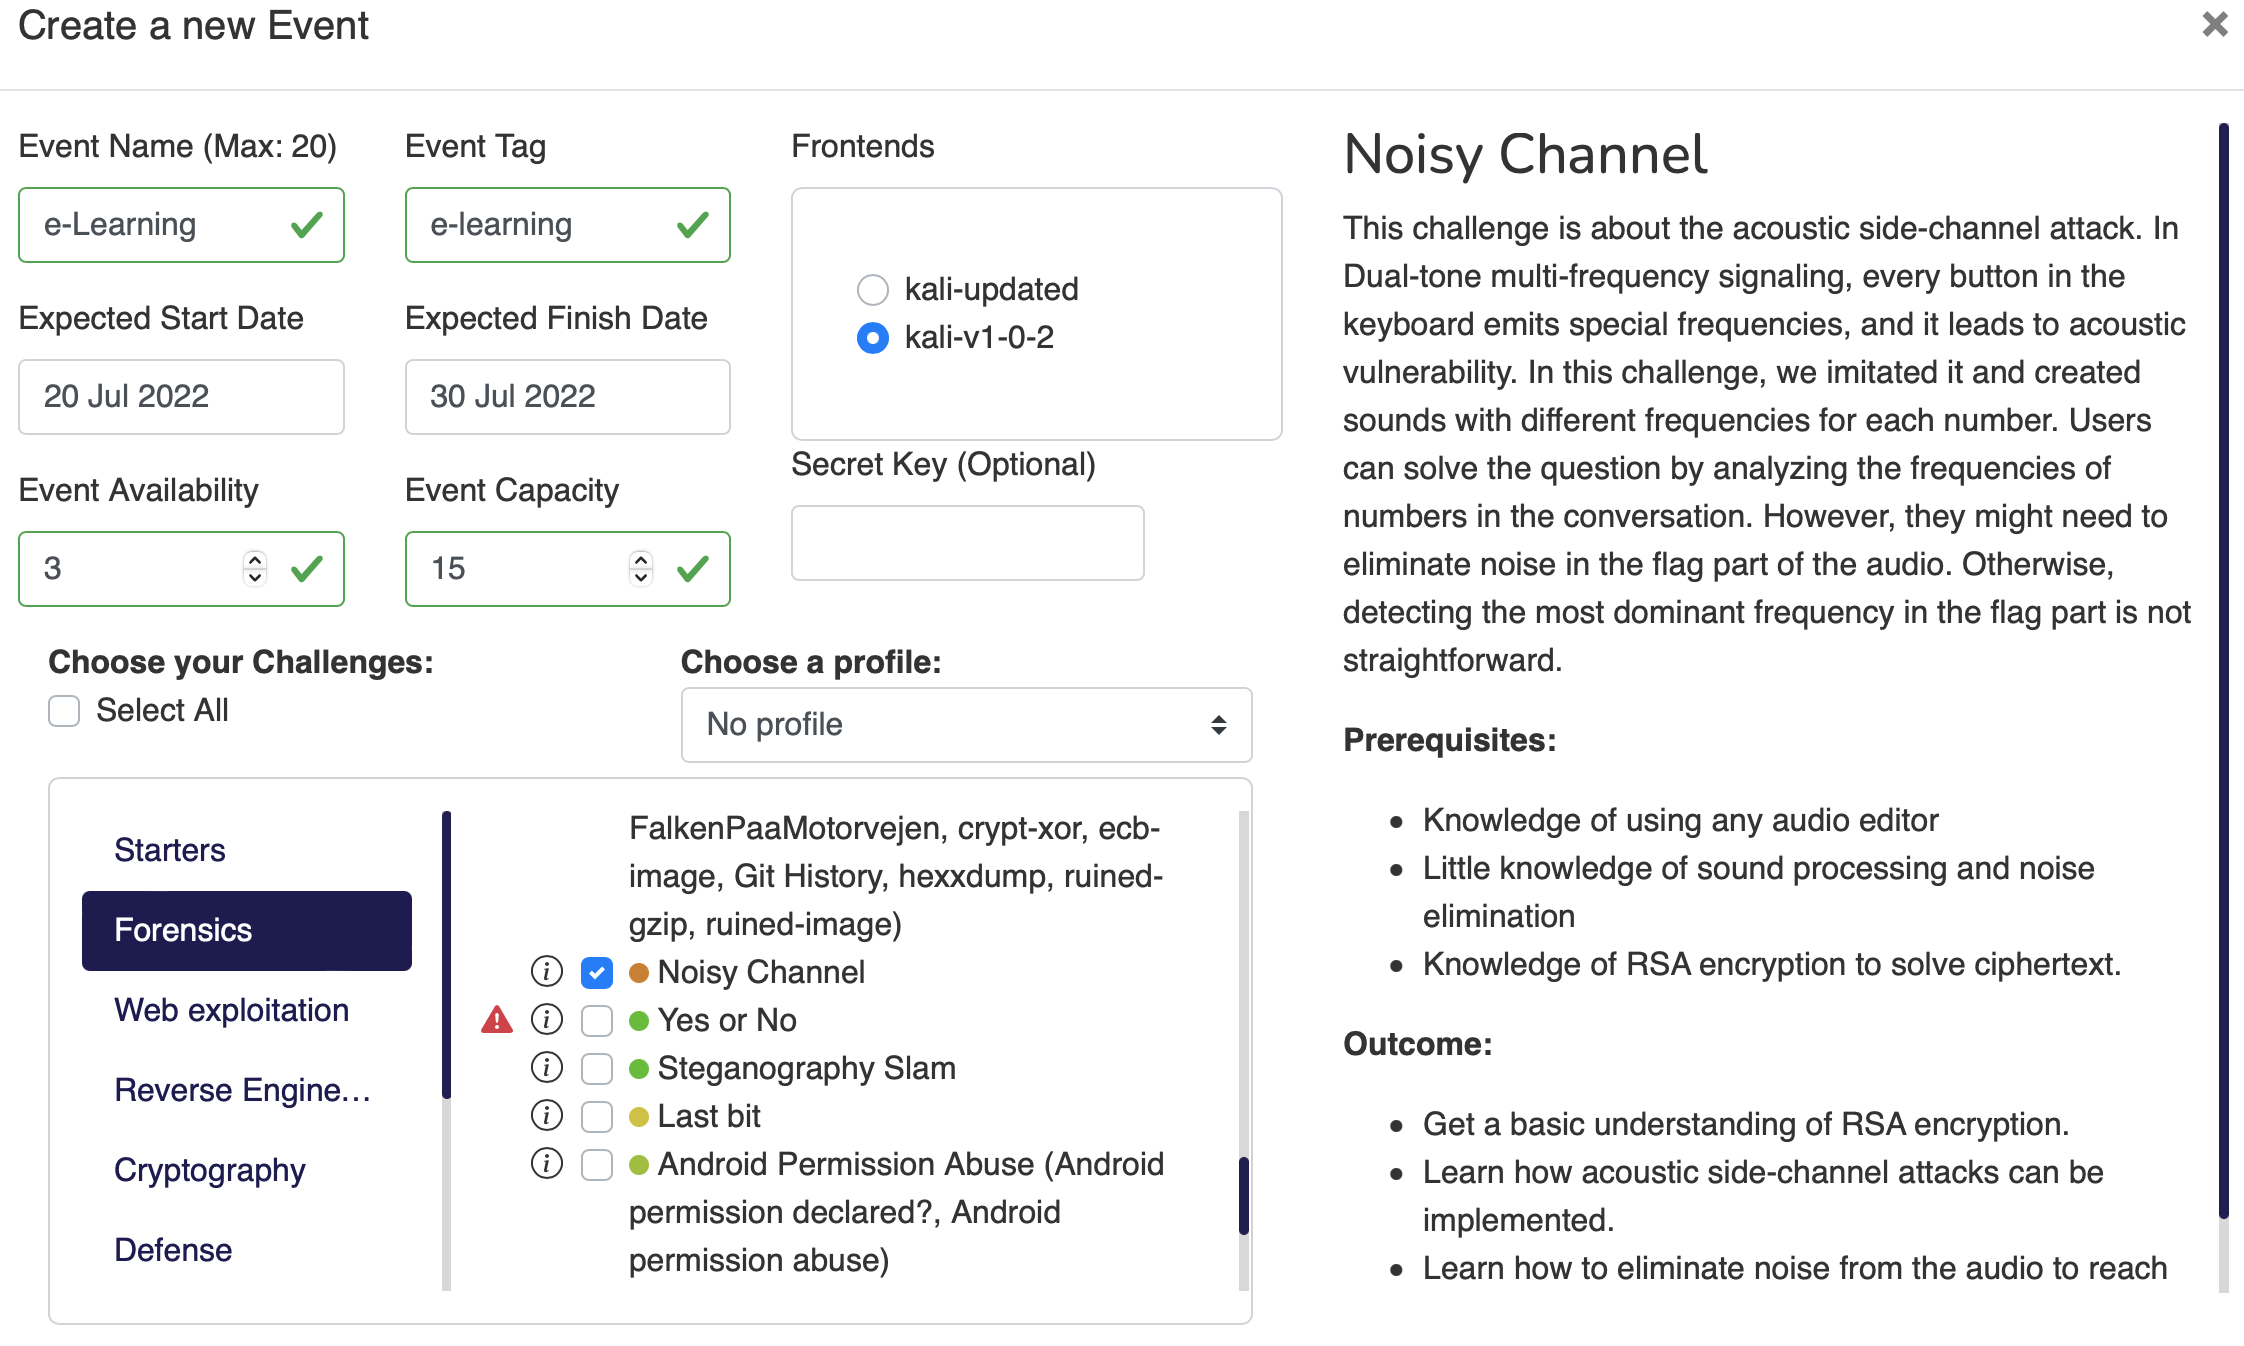
\includegraphics[scale=.4]{figures/web-interface.png}}
\caption[Event creation using web interface]{Event creation using web interface \footnote{https://admin.haaukins.com:8003}}
\label{fig}
\end{figure}

Figure 4.3 represents creation step of an event with detailed fields. Administrators and instructors can create events specifically on particular topic. In left corner side of the figure, categories of the challenges are listed, each category has at least thirty challenges and increases as time pass. When selecting set of challenges, all information about a challenge can be checked in right side of the figure. The fields (Event Name, Event Tag and all others ) reveals extra information when hover on them. 
There are tons of new, user friendly and supportive features for leveraging the platform's capabilities. It substantially aids  instructors to have valuable challenges in the event parallel to their circular.

Administration of the platforms are people who are running the platform at Aalborg University. However, an instructor signs up for their usage, both administrators and instructors can have similar management permissions except few permissions.
It is possible to manage events on behalf of event creators or event creators can manage their events through web interface. 

\begin{figure}[htbp]
\centerline{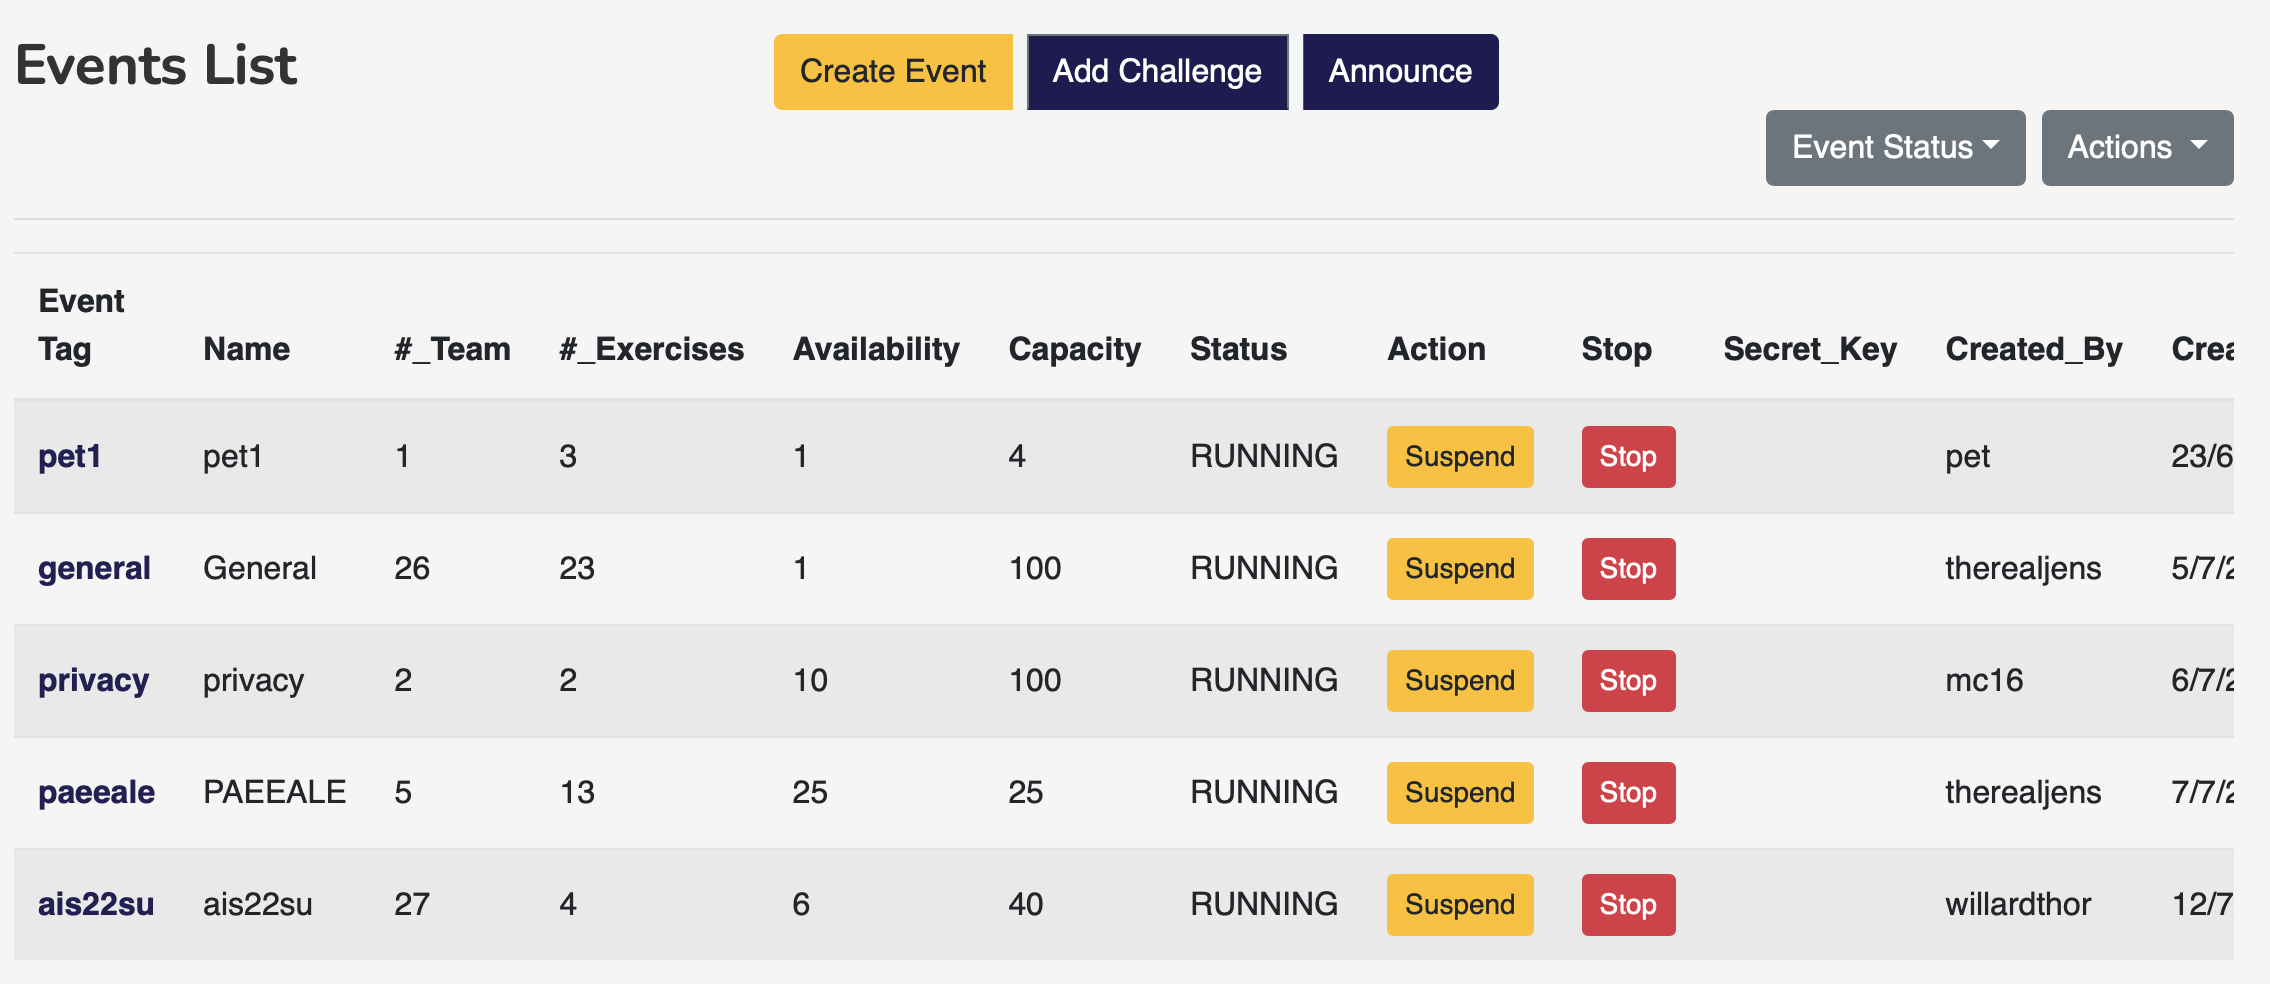
\includegraphics[scale=.4]{figures/events_list.png}}
\caption[Listing events on web client of Haaukins platform ]{Listing events on web client of Haaukins platform\footnote{https://admin.haaukins.com:8003}}
\label{fig}
\end{figure} 

Figure 4.4 represents possible actions that an authorized person can take either on their event only, or all events depending of their role. Event tag represents subdomain, for instance event called "general" runs at general.haaukins.com, "privacy" runs at privacy.haaukins.com 
An even can be suspended for some time, stopped manually. All students/teams can be managed in an event through web client, if a challenge is forgotten in case of event creation. It can be added afterwards and the platform will propagate resource allocation and assignment of the challenges to the event participants. 

There are many other features and capabilities of the platform. The web client delivers all those features in a user-friendly, informative and easy to understand structure. All developments are done in a feedback loop from users of the platform. As usage of it increased in educational institutions, the platform became better and better. 

Finally, there are still ongoing feature requests and improvements at Github\footnote{https://github.com/aau-network-security/haaukins-webclient}. Since all Haaukins and its services are open source, it is possible to deploy and modify according to your requirements. There is high lack of having this flexibility on practical security education. 



